\documentclass[
fontsize=12pt, 
paper=a4, 
BCOR=10mm, 
twoside=false,
 DIV=10, 
 headsepline, 
 footsepline
 ]{scrartcl} 
 
 %%________________________________________________________

% 1,5 facher ZeilenAbstand
\usepackage[onehalfspacing]{setspace}
%\usepackage[singlespacing]{setspace}
%\usepackage[doublespacing]{setspace}
%
%oder man nehme \linespread{value}
%
%where value determine line spacing. This value is somewhat confusing, because:
%
%Value	Line spacing
%1.0		single spacing
%1.3		one-and-a-half spacing
%1.6		double spacing

% Bindungskorrektur papierverlust durch Hefter 7,5 und durchs knicken 0,75
%\KOMAoptions{BCOR=8.25mm}
%%________________________________________________________

\AfterTOCHead{\singlespacing} %Nach der Überschrift des Inhaltsverzeichnisses wird ein \\gesetzt


%Neue Satztspiegelberchenen
\recalctypearea
\KOMAoptions{DIV=last}

%\KOMAoptions{headsepline}
%\KOMAoptions{footsepline}

\usepackage[autooneside=true]{scrlayer-scrpage}
\pagestyle{scrheadings}
%\lohead{}
%\rohead{Daniel Ludwig}
%\lofoot{HAW Hamburg}
\setkomafont{pageheadfoot}{\small} % Aufrechte und kleine Schrift in header und foot
\automark[subsection]{section}

%Kollumnentitel (Section) wird links in den Header geschrieben, mit Stern
%\ihead*{\headmark}
%\ohead{Daniel Ludwig}

%Wer das Dokument nicht mit KOMA/typeare nach Satzspiegel formatieren möchte
% nutzt 
\usepackage{geometry}                		
\geometry{a4paper}                   		% ... or a4paper or a5paper or ... 
%\geometry{landscape}                		% Activate for rotated page geometry
%\usepackage[parfill]{parskip}    		% Activate to begin paragraphs with an empty line rather than an indent
% \geometry{
% left = 3cm,
% right = 2cm,
% top = 2cm
% bottom = 2cm}


\usepackage[english,ngerman]{babel} % Die letzte angegebene Sprache wird als Hauptsprache festgelegt.

\usepackage[utf8]{inputenc} %UTF-8 Codierung (Umlaute etc.; Deutsch, Englisch, Portugiesisch...)
%\usepackage[T1]{fontenc} % zum nutzen von pdfLaTeX

%Schrifttyp
%\setmainfont{QTCaslan}
%\setmainfont{Arno Pro}

%%________________________________________________________ 
%%________________________________________________________ 

\usepackage{fontspec} %Um installierte fonts mit XeTeX zu nutzen

%Serifen Schiften
%_____________________________________________________________________________
%
\setromanfont{Arno Pro}
%\setromanfont{Century Schoolbook}
%\setromanfont{PT Serif}

%Serifenlose Schiften
%_____________________________________________________________________________

\setsansfont{Hypatia Sans Pro}
%\setsansfont{Hypatia Sans Pro}
%\setsansfont{Futura}
%\setsansfont{PT Sans}

%Typewriter (Programmiercode, Hyperref) Schiften
%_____________________________________________________________________________
%\setmonofont[Color={0019D4},Scale=0.85]{Special Elite}
%\setmonofont[Scale=0.9]{Special Elite}
%\setmonofont[Color={0019D4},Scale=1]{Lucida Grande}
\setmonofont[Color={0019D4},Scale=.8]{Menlo}
%\setmonofont[Color={0019D4},Scale=.8]{Andale Mono}
%\setmonofont[Color={0019D4}]{RM Typerighter}
%\setmonofont[Color={0019D4}]{Courier New} %Typewriter/Schreibmaschinen Schrift in Blau 

%Progammcode/Typewriter Umgebung
%\begin{verbatim}
%usually this environment is used to display code
%\end{verbatim}


\usepackage{geometry}                		
\geometry{a4paper}                   		% ... or a4paper or a5paper or ... 
%\geometry{landscape}                		% Activate for rotated page geometry
%\usepackage[parfill]{parskip}    		% Activate to begin paragraphs with an empty line rather than an indent

\usepackage{graphicx}				% Use pdf, png, jpg, or eps§ with pdflatex; use eps in DVI mode

\usepackage[table,xcdraw]{xcolor}				
\usepackage{caption}								
\usepackage{float}
\usepackage{amssymb}
\usepackage{pdfpages}
%\usepackage{parskip}
\usepackage{siunitx}
\usepackage{amsmath}
\usepackage{longtable}
\usepackage{tabularx}
\usepackage{colortbl}

%___________________________________________________________________________
%___________________________________________________________________________

\usepackage{varwidth}
%\begin{figure}[h!]
%\centering
%\begin{varwidth}{\linewidth}
%\begin{verbatim}
%'\s\+\s\s\s\s12\.8\sg\s\r\n'
%\end{verbatim}
%\end{varwidth}
%\end{figure}
%___________________________________________________________________________

\usepackage{fancyvrb}
%\begin{figure}[h!]
%\centering
%\begin{BVerbatim}
%'\s''\+''\s''\s''\s''\s''12''\.''8''\s''g''\s''\r''\n'
%\end{BVerbatim}
%\end{figure}
%___________________________________________________________________________%___________________________________________________________________________

\usepackage{tikz}
\usetikzlibrary{chains}

%%Bibtex JabRef *.bib Datei
%__________________________________________________________________
\bibliographystyle{unsrt}
\usepackage[backend=biber]{biblatex}
\addbibresource{Masterthesis_Literaturverzeichnis.bib} 
%__________________________________________________________________

%\usepackage{subcaption}



\usepackage{mwe}    % loads »blindtext« and »graphicx«
\usepackage{subfig}
 
\begin{document}
   \begin{figure}[!ht]
     \subfloat[][\texttt{true}\label{fig:true}]{%
       \includegraphics[width=0.48\textwidth]{Bilder/LabVIEW_serialport/step7_elapsed_true.jpg}
     }
     \hfill     
     \subfloat[][\texttt{false}\label{fig:false}]{%
       \includegraphics[width=0.48\textwidth]{Bilder/LabVIEW_serialport/step7_elapsed_false.jpg}
     }
     \caption{Methode 2 Elapsed Time \\     	\textbf{links} \glqq \texttt{true}\grqq{} (37)  \, \, 
     %\hspace{20pt}
 		\textbf{rechts}  \glqq \texttt{false}\grqq{} (37)
  }
  \label{fig:elapsed_time}
   \end{figure}
   
   
   
   
   
   
%   \begin{figure}
%     \centering
%%
%     \begin{subfigure}[a]{width=0.4\textwidth}
%         \centering
%         \includegraphics[width=0.4\linewidth]{%
%         Bilder/LabVIEW_serialport/step7_elapsed_true.jpg}
%%         \caption{\texttt{true}}
%%         \label{fig:true}
%     \end{subfigure}
%     \hfill
%%
%     \begin{subfigure}[b]{width=0.4\textwidth}
%         \centering
%         \includegraphics[width=0.4\linewidth]{%
%         Bilder/LabVIEW_serialport/step7_elapsed_false.jpg}
%%         \caption{\texttt{false}}
%%         \label{fig:false}
%     \end{subfigure}
%     \hfill
%     \caption{Methode 2 \\
%  \textbf{links} \glqq Elapsed Time\grqq{} (37) \texttt{false} \\
%  \textbf{rechts}  \glqq Elapsed Time\grqq{} (37) \texttt{true}
%  }
%  \label{fig:elapsed_time}
%\end{figure}


\end{document}




\usepackage{subfig} %zwei Bilder nebeneinander
%\begin{figure}%
%  \centering
%  \subfloat[][]{\includegraphics[width=0.4\linewidth]{ozean}}%
%  \qquad
%  \subfloat[][]{\includegraphics[width=0.4\linewidth]{cow}}%
%  \caption{Zu Wasser und zu Land}
%	 \label{}
%\end{figure}

% Makro bild
% #1 : Skalierungsfaktor | width=#1\textwidth
% #2 : Grafikdatei.png
% #3 : Abstand zwischen Grafik Bildunterschrift | 1em ist ein Abstand der Breite eines 		 			großen M dieser Schriftgröße
% #4 : Bildunterschrift
% #5 : Verweis-Label

\def\bild#1#2#3#4#5#6{%
\begin{figure}[h!] %[htbp!] bedeutet here top bottom page und das ! bedeutet die Begrenzungen von Latex aufzuheben
\centering
\includegraphics[width=#1\textwidth]{Bilder/#2}
\vspace{#3}
\caption[#4]{#5}\label{#6}
\end{figure}
}
%Ergebnis: \bild{0.8}{template-1.png}{-1em}{Eine Kr¨ote oder ein Frosch}{fig:1}

%Inhaltsangabentiefenformatierung
%__________________________________________________________________

\setcounter{tocdepth}{4}
%__________________________________________________________________


%Paragraph verhält sich wie die vierte Ebene (subsubsubsection)
%__________________________________________________________________
%\setcounter{secnumdepth}{4}











\begin{document} 



%Seitenzähler reset mit große römische Ziffern
%%_____________________________________________________________________
%\pagenumbering{Roman}
%%_____________________________________________________________________


%\usepackage{acronym}

%\begin{acronym} 
%
%%\ac{abktag}   abkürzung wird eingeführt
%%\acs{abktag} Abkürzung wird nicht eingeführt
%%\acl{abktag} gibt die ausgeschriebene Form aus
%
%\acro{KI}[KI]{künstliche Intelligenz} 
%\acro{mvt}[mvt]{mechanische Verfahrenstechnik}
%
%\end{acronym}

% Wörter untrennbar machen:
% \mbox{}


%
%\begin{figure}%
%  \centering
%  \subfloat{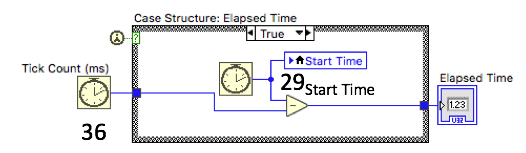
\includegraphics[width=0.4\linewidth]{%
%  LabVIEW_serialport/step7_elapsed_true.png}}%
%  \qquad
%  \subfloat{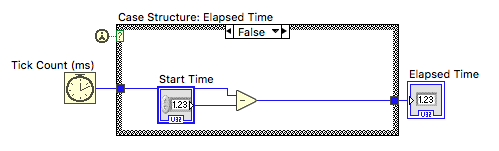
\includegraphics[width=0.4\linewidth]{%
%  LabVIEW_serialport/step7_elapsed_false.png}}%
% % \vspace{0em}
%  \caption{Methode 2 \\
%  \textbf{links} \glqq Elapsed Time\grqq{} (37) \texttt{false} \\
%  \textbf{rechts}  \glqq Elapsed Time\grqq{} (37) \texttt{true}
%  }
%	 \label{elapsed_time}
%\end{figure}





\section*{test}
\begin{figure}
     \centering
%
     \begin{subfigure}[a]{width=0.4\textwidth}
         \centering
         \includegraphics[width=0.4\linewidth]{%
         LabVIEW_serialport/step7_elapsed_true.jpg}
%         \caption{\texttt{true}}
%         \label{fig:true}
     \end{subfigure}
     \hfill
%
     \begin{subfigure}[b]{width=0.4\textwidth}
         \centering
         \includegraphics[width=0.4\linewidth]{%
         LabVIEW_serialport/step7_elapsed_false.jpg}
%         \caption{\texttt{false}}
%         \label{fig:false}
     \end{subfigure}
     \hfill
     \caption{Methode 2 \\
  \textbf{links} \glqq Elapsed Time\grqq{} (37) \texttt{false} \\
  \textbf{rechts}  \glqq Elapsed Time\grqq{} (37) \texttt{true}
  }
  \label{fig:elapsed_time}
\end{figure}

\end{document} 